

\documentclass{beamer}

\mode<presentation> {

% The Beamer class comes with a number of default slide themes
% which change the colors and layouts of slides. Below this is a list
% of all the themes, uncomment each in turn to see what they look like.

%\usetheme{default}
%\usetheme{AnnArbor}
%\usetheme{Antibes}
%\usetheme{Bergen}
%\usetheme{Berkeley}
%\usetheme{Berlin}
%\usetheme{Boadilla}
%\usetheme{CambridgeUS}
%\usetheme{Copenhagen}
%\usetheme{Darmstadt}
%\usetheme{Dresden}
%\usetheme{Frankfurt}
%\usetheme{Goettingen}
%\usetheme{Hannover}
%\usetheme{Ilmenau}
%\usetheme{JuanLesPins}
%\usetheme{Luebeck}
%\usetheme{Madrid}
%\usetheme{Malmoe}
%\usetheme{Marburg}
%\usetheme{Montpellier}
%\usetheme{PaloAlto}
%\usetheme{Pittsburgh}
%\usetheme{Rochester}
%\usetheme{Singapore}
%\usetheme{Szeged}
%\usetheme{Warsaw}

% As well as themes, the Beamer class has a number of color themes
% for any slide theme. Uncomment each of these in turn to see how it
% changes the colors of your current slide theme.

%\usecolortheme{albatross}
%\usecolortheme{beaver}
%\usecolortheme{beetle}
%\usecolortheme{crane}
%\usecolortheme{dolphin}
%\usecolortheme{dove}
%\usecolortheme{fly}
%\usecolortheme{lily}
%\usecolortheme{orchid}
%\usecolortheme{rose}
%\usecolortheme{seagull}
%\usecolortheme{seahorse}
%\usecolortheme{whale}
\usecolortheme{wolverine}

%\setbeamertemplate{footline} % To remove the footer line in all slides uncomment this line
%\setbeamertemplate{footline}[page number] % To replace the footer line in all slides with a simple slide count uncomment this line

%\setbeamertemplate{navigation symbols}{} % To remove the navigation symbols from the bottom of all slides uncomment this line
}

\usepackage{graphicx} % Allows including images
\usepackage{booktabs} % Allows the use of \toprule, \midrule and \bottomrule in tables


\usepackage{listings}
\lstset{language=Java,
                basicstyle=\footnotesize\ttfamily,
                keywordstyle=\footnotesize\color{blue}\ttfamily,
}

%----------------------------------------------------------------------------------------
%	TITLE PAGE
%----------------------------------------------------------------------------------------

\title[Java]{1.Very first introduction to java} % The short title appears at the bottom of every slide, the full title is only on the title page

\author{Sakib Abrar} % Your name
\institute[BUET] % Your institution as it will appear on the bottom of every slide, may be shorthand to save space
{
CSE\\~\\Bangladesh University of Engineering \& Technology \\ % Your institution for the title page
\medskip
\textit{sakib.cghs@gmail.com} % Your email address
}
\date{\today} % Date, can be changed to a custom date

\begin{document}

\begin{frame}
\titlepage % Print the title page as the first slide
\end{frame}

\begin{frame}
\frametitle{Overview} % Table of contents slide, comment this block out to remove it
\tableofcontents % Throughout your presentation, if you choose to use \section{} and \subsection{} commands, these will automatically be printed on this slide as an overview of your presentation
\end{frame}

%----------------------------------------------------------------------------------------
%	PRESENTATION SLIDES
%----------------------------------------------------------------------------------------

%------------------------------------------------
\section{What is Java?}
%------------------------------------------------

\begin{frame}
\frametitle{Java}
A simple, object‐oriented, distributed, interpreted,
robust, secure, architecture neutral, portable,
high‐performance, multithreaded, and dynamic
language ‐‐ Sun Microsystems.\\~\\
It is a powerful general-purpose programming language. It is used to develop desktop and mobile applications, web applications, big data processing, embedded systems, and so on.\\~\\
Java syntax is similar to C++, but is strictly an object-oriented programming language. \\~\\

\end{frame}

%------------------------------------------------
\section{Why should you learn Java?}
%------------------------------------------------

\begin{frame}
\frametitle{Why Java?}
\begin{itemize}
\item Java is highly popular!!
\item It is Versatile
\item It is also Platform Independent
\item Lots of Powerful Development Tools
\item Java has a Large Community
\item Great Documentation Support
\item Java has multiple Open Source Libraries
\item Last but not the least High Salary!!

\end{itemize}
\end{frame}

%-----------------------------------------------
\section{How to setup development environment for java?}
%------------------------------------------------

\begin{frame}
\frametitle{Softwares we need}
\vspace{0.2in}
\centerline{\huge{Two things to get set up}}
\vspace{0.2in}
\begin{block}{1.JDK}
Java development kit.\\~\\

\includegraphics[width=0.2\textwidth]{jdk.png}
\end{block}
\begin{block}{2.IDE}
Integrated Development Environment(java supported).\\~\\

\includegraphics[width=0.15\textwidth]{ide1.png} \vspace{1cm}   
\includegraphics[width=0.15\textwidth]{ide2.png} \vspace{1 		cm}  
\includegraphics[width=0.15\textwidth]{ide3.png}
\end{block}
\end{frame}

%-----------------------------------------------
\section{Our very first java program?}
%-----------------------------------------------

\begin{frame}[fragile]{First java program}
Create and open a project in Intellij then create a new java class named FirstProgram.java then type\\~\\
\begin{columns}[T]
% code
\begin{column}{\textwidth}
\begin{lstlisting}
public class FirstProgram {
    public static void main(String[] args) {
        System.out.println("Hello World");
    }
}
\end{lstlisting}
\end{column}
% description
\end{columns}
\vspace{0.4in} Then hit run and see!
\end{frame}


%-----------------------------------------------
\section{Examining the java file}
%------------------------------------------------

\begin{frame}
\frametitle{Examining FirstProgram.java}
\textbf{public static void main(String[] args)}
\begin{itemize}
\item \textbf{main} is the starting point of every Java application
\item \textbf{public} is used to make the method accessible by all
\item \textbf{static} is used to make main a static method of class
Welcome. Static methods can be called without using any
object; just using the class name. JVM call main using the
\textbf{ClassName.methodName} FirstProgram.main ) notation
\item \textbf{void} means main does not return anything
\item \textbf{String args[]} represents an array of String objects that
holds the command line arguments passed to the
application. Where is the length of args array?
\end{itemize}
\end{frame}

%------------------------------------------------

\begin{frame}
\frametitle{Examining FirstProgram.java}
\textbf{System.out.println}
\begin{itemize}
\item Used to print a line of text followed by a new line
\item \textbf{System}  is a class inside the Java API
\item \textbf{out} is a public static member of class System
represents the standard output (similar to C/C++ stdout or cout)
\item\textbf{println} is a public method of the class of which out is an object
\end{itemize}
\end{frame}

%-----------------------------------------------
\section{Basic Overview of java}
%------------------------------------------------

\begin{frame}
\frametitle{Java Basics}
\begin{itemize}
\item Everything should reside under a class(or probably many classes)
\item The source file name must match the name of the public class defined in the file with the .java extension
\item A Java source file can contain multiple classes, but only one class can be a public class

\end{itemize}
\end{frame}


%-----------------------------------------------
\section{How does it work?}
%------------------------------------------------

\begin{frame}
\frametitle{How java works}
\huge{\centerline{JDK got your back!!}}
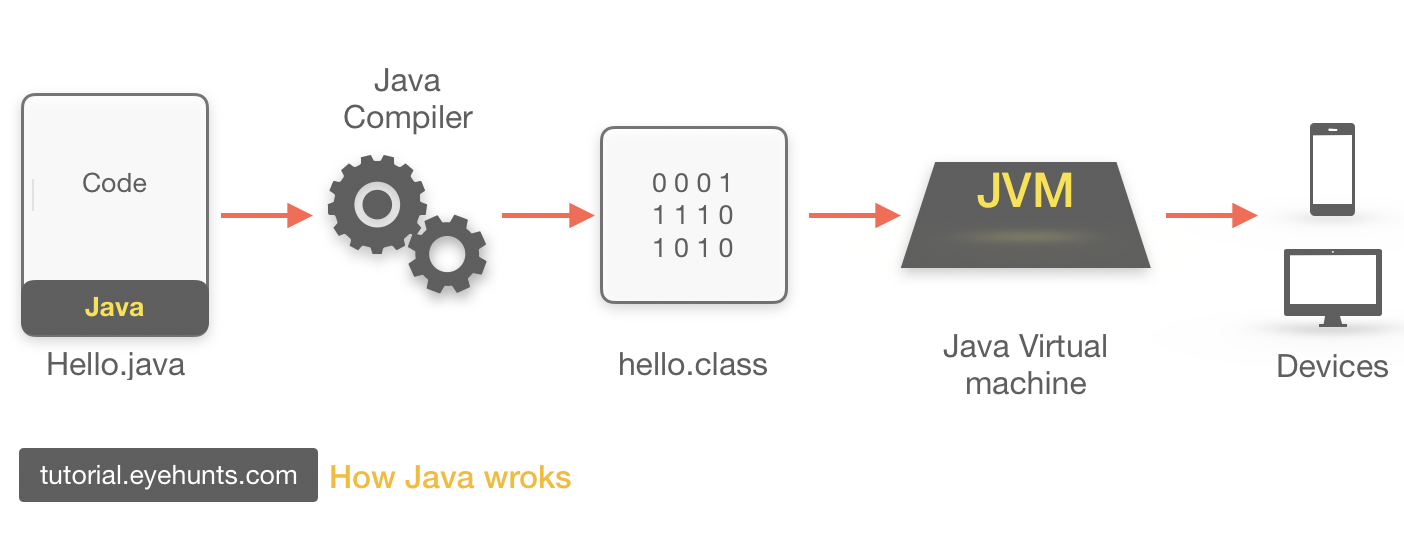
\includegraphics[width=\textwidth]{howitworks.png}
\end{frame}


%---------------------------------------------------------------------------------------

\begin{frame}
\Huge{\centerline{The End}}
\end{frame}

%----------------------------------------------------------------------------------------

\end{document} 